%%%%%%%%%%%%%%%%%%%%%%%%%%%%%%%%%%%%%%%%%%%%%%%%%%%
%% LaTeX book template                           %%
%% Author:  Amber Jain (http://amberj.devio.us/) %%
%% License: ISC license                          %%
%%%%%%%%%%%%%%%%%%%%%%%%%%%%%%%%%%%%%%%%%%%%%%%%%%%

\documentclass[a4paper,11pt]{book}

\usepackage[T1]{fontenc}
\usepackage[utf8]{inputenc}
\usepackage{lmodern}
\usepackage{hyperref}
\usepackage{graphicx}
\usepackage[portuguese]{babel}
\usepackage{amsfonts}
\usepackage[usenames,dvipsnames]{xcolor}
\usepackage{mathtools}
\usepackage{amssymb} % alguns simbolos matematicos
\usepackage{ mathrsfs } % letras cursivas

% para usar definições
\usepackage{amsthm}

\theoremstyle{definition}
\newtheorem{definition}{Definition}[section]

% tirando identação dos paragrafos
\setlength{\parindent}{0ex}

% coding examples in latex file
\usepackage{listings}
\usepackage{xcolor}

\definecolor{codegreen}{rgb}{0,0.6,0}
\definecolor{codegray}{rgb}{0.5,0.5,0.5}
\definecolor{codepurple}{rgb}{0.58,0,0.82}
\definecolor{backcolour}{rgb}{0.95,0.95,0.92}

\lstdefinestyle{mystyle}{
    backgroundcolor=\color{backcolour},   
    commentstyle=\color{codegreen},
    keywordstyle=\color{magenta},
    numberstyle=\tiny\color{codegray},
    stringstyle=\color{codepurple},
    basicstyle=\ttfamily\footnotesize,
    breakatwhitespace=false,         
    breaklines=true,                 
    captionpos=b,                    
    keepspaces=true,                 
    numbers=left,                    
    numbersep=5pt,                  
    showspaces=false,                
    showstringspaces=false,
    showtabs=false,                  
    tabsize=2
}

\lstset{style=mystyle}

%%%%%%%%%%%%%%%%%%%%%%%%%%%%%%%%%%%%%%%%%%%%%%%%%%%%%%%%%%%%%%%%%%%%%%%%%%%%%%%%
% 'dedication' environment: To add a dedication paragraph at the start of book %
% Source: http://www.tug.org/pipermail/texhax/2010-June/015184.html            %
%%%%%%%%%%%%%%%%%%%%%%%%%%%%%%%%%%%%%%%%%%%%%%%%%%%%%%%%%%%%%%%%%%%%%%%%%%%%%%%%
\newenvironment{dedication}
{
   \cleardoublepage
   \thispagestyle{empty}
   \vspace*{\stretch{1}}
   \hfill\begin{minipage}[t]{0.66\textwidth}
   \raggedright
}
{
   \end{minipage}
   \vspace*{\stretch{3}}
   \clearpage
}

%%%%%%%%%%%%%%%%%%%%%%%%%%%%%%%%%%%%%%%%%%%%%%%%
% Chapter quote at the start of chapter        %
% Source: http://tex.stackexchange.com/a/53380 %
%%%%%%%%%%%%%%%%%%%%%%%%%%%%%%%%%%%%%%%%%%%%%%%%
\makeatletter
\renewcommand{\@chapapp}{}% Not necessary...
\newenvironment{chapquote}[2][2em]
  {\setlength{\@tempdima}{#1}%
   \def\chapquote@author{#2}%
   \parshape 1 \@tempdima \dimexpr\textwidth-2\@tempdima\relax%
   \itshape}
  {\par\normalfont\hfill--\ \chapquote@author\hspace*{\@tempdima}\par\bigskip}
\makeatother


%%%%%%%%%%%%%%%%%%%%%%%%%%%%%%%%%%%%%%%%%%%%%%%%%%%
% First page of book which contains 'stuff' like: %
%  - Book title, subtitle                         %
%  - Book author name                             %
%%%%%%%%%%%%%%%%%%%%%%%%%%%%%%%%%%%%%%%%%%%%%%%%%%%
% Book's title and subtitle
\title{\Huge \textbf{Book of Proof} \\ 
\huge Third Edition}
% Author
\author{\textsc{Richard Hammack}}


\begin{document}

\frontmatter
\maketitle

\tableofcontents
%\listoffigures
%\listoftables

\mainmatter


\part{Fundamentos}

%%%%%%%%%%%%%%%%%%%%%%%%%%%%%%%%%%%%%%%%%%%%%%%%%%%
%                 CHAPTER                         %
%%%%%%%%%%%%%%%%%%%%%%%%%%%%%%%%%%%%%%%%%%%%%%%%%%%
\chapter{Conjuntos}


\begin{chapquote}{página 3}
	``The theory of sets is a language that is perfectly suited to describing and explaning all types of mathematical structures.''
\end{chapquote}


\section{Introdução}
Um \textbf{conjunto} (set) é uma lista de \textbf{elementos}. Normalmente denotados por uma letra maiúscula. Por exemplo:

\begin{center}
	$ A = \{1 , 2 , 3 , 4 , ... \} $
\end{center}

Dois sets $A$ e $B$ são \textbf{iguais} se possuírem exatamente os mesmos elementos. Não importando a ordem desses elementos dentro de cada set.
\\
\\
Vamos definir um símbolo para sinalizar se um determinado elemento $(x)$ pertence ou não a um determinado set qualquer $(A)$. Para tal relação usaremos o símbolo $``\in"$ se $x$ for um elemento de $A$ ou, caso contrário, usaremos $``\notin"$ se $x$ não for um elemento de $A$.
\\
\\
É provável que, em algum momento, seja necessário contar a quantidade de elementos em um dado set qualquer $A$. Chamaremos essa relação de \textbf{cardinalidade} ou \textbf{tamanho} do set $A$. O símbolo usado será duas barras em volta do set do seguinte modo: $``|A|"$.
\\
\\
A partir dessas duas relações já podemos definir um tipo especial de set. Vamos definir como \textbf{conjunto vazio} ou \textbf{empty set} um conjunto que possua o cardinal igual a zero. Usaremos o símbolo $``\emptyset"$ para definir a relação abaixo:

\begin{center}
	$|\emptyset| = 0$
\end{center}

Em várias situações não vale a pena construir sets apenas com uma lista de alguns dos seus elementos. Imagine um set de todos os números pares, por exemplo, ou um set de todos os números que começam com $3$ e terminam com $4$ ou qualquer outra regra mais específica. Para essas situações usamos a \textbf{notação de formação de conjuntos (set builder notation)}. Como no exemplo abaixo:

\begin{center}
	$ E = $ \textcolor{red}{$\{$} \textcolor{blue}{$2n$} \textcolor{OliveGreen}{$:$} \textcolor{Brown}{$n$} \textcolor{Orange}{$\in$} $\mathbb{Z} \}$
\end{center}

A matemática é uma linguagem que consegue dizer muita coisa com poucos símbolos. Ao longo desse curso, você será capaz de ler esses símbolos e compreender corretamente o que o autor quis dizer por meio deles. Para facilitar essa primeira leitura, eu colori cada símbolo da expressão acima com a cor correspondente da passagem a seguir. Perceba como um pequeno símbolo pode significar bastante coisa. A leitura da expressão acima é: "O conjunto $E$ é igual ao \textcolor{red}{conjunto dos elementos da forma} \textcolor{blue}{$2n$} \textcolor{OliveGreen}{tal que} \textcolor{Brown}{$n$} \textcolor{Orange}{é um elemento do conjunto} $\mathbb{Z}$".
\\
\\
Podemos resumir essa notação de formação de conjuntos como "$Conjunto = \{ Expressão : Regra \}$". É bem comum vermos notações onde os dois pontos são trocados por uma barra: "$Conjunto = \{ Expressão \ | \ Regra \}$".
\\
\\
Existem alguns conjuntos que são famosos ao ponto de terem nomes e símbolos próprios.
\begin{itemize}
	\item[] $\emptyset = \{ \}$
	\item[] $\mathbb{N} = \{ 1, 2, 3, 4, ... \}$, perceba que $0 \notin \mathbb{N}$
	\item[] $\mathbb{Z} = \{ ..., -2, -1, 0, 1, 2, ...  \}$
	\item[] $\mathbb{Q} = \{ x : x = m/n, \ onde \ m,n \in \mathbb{Z} \  e \  n \neq 0 \}$
	\item[] 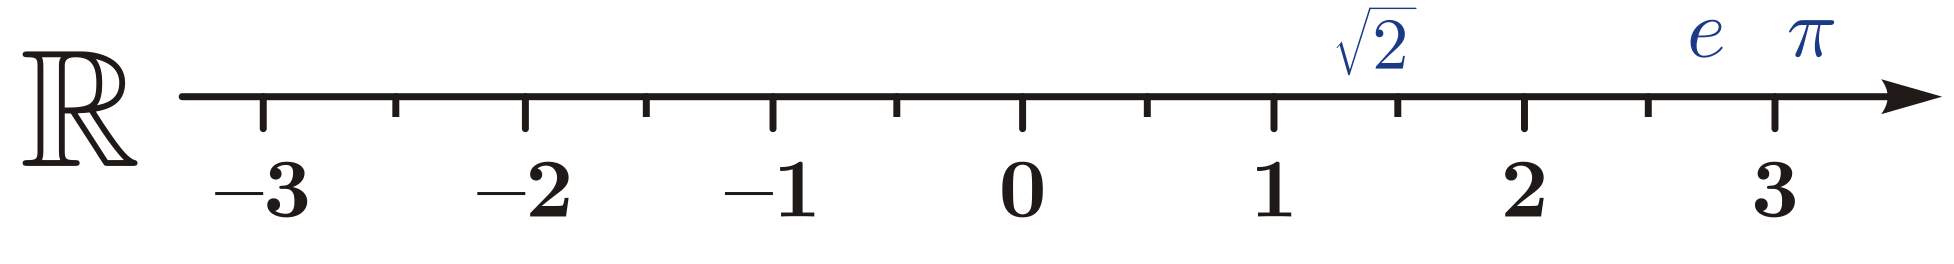
\includegraphics[scale=0.11]{images/real_line.png}
\end{itemize}

Como o conjunto dos número reais pode ser descrito como pontos em uma reta numérica infinita. Se tivermos dois pontos quaisquer $a$ e $b$, de modo que $a$ e $b \in \mathbb{R}$ e $a < b$. Temos infinitos elementos entre esses dois pontos. Por causa dessa propriedade, teremos que usar um novo símbolo para se referir aos conjuntos que são melhor descritos em termos de \textbf{intervalos} entre pontos. Abaixo coloquei uma coluna com uma representação gráfica e, ao lado, uma coluna com a respectiva definição por set builder notation.
\begin{center}
	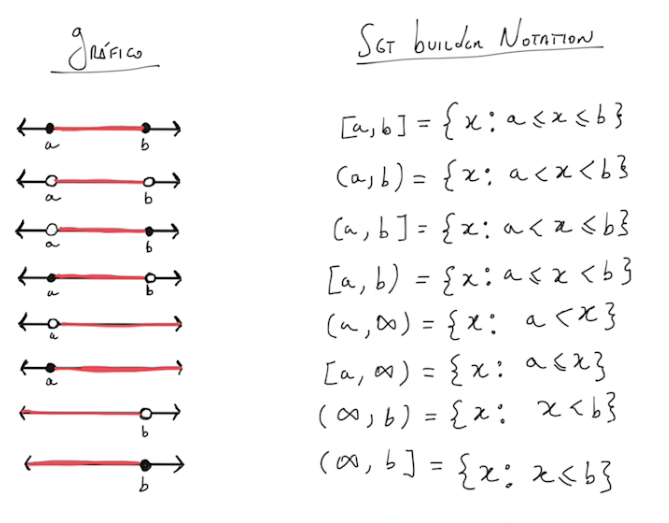
\includegraphics[scale=0.7]{images/intervals.png}
\end{center}

\section{Produto Cartesiano}
\begin{definition}[Par Ordenado]
Um \textbf{par ordenado} é um lista na forma $(x, y)$ que contém dois elementos (nesse caso, um $x$ e um $y$). Onde esses dois elementos estão entre parênteses e separados por uma vírgula.
\end{definition}

\textbf{Atenção}: Atente para o fato que $(x,y) \neq (y,x)$. 
\\
\\
Agora que temos a definição de par ordenado. Podemos escrever conjuntos usando esse novo conceito.

\begin{definition}[Produto Cartesiano]
O \textbf{produto cartesiano} de dois sets $A$ e $B$ é um outro set cujo símbolo é $``A \times B"$ e é definido como:
\begin{center}
$A \times B = \{ (a,b) : a \in A, b \in B \}$
\end{center}
\end{definition}

Perceba que, se $A$ e $B$ são finitos, então $| A \times B | = |A| . |B|$ (ou seja, o cardinal do produto cartesiano de dois sets é igual à multiplicação dos cardinais dos dois conjuntos).
\\
\\
Podemos construir um produto cartesiano onde os conjuntos $A$ e $B$ são iguais. Por exemplo: $\mathbb{R} \times \mathbb{R} = \{ (x,y) : x,y \in \mathbb{R} \}$.
\\
\\
Para simplificar essa expressão onde temos um produto cartesiano de sets iguais, vamos criar um novo conceito que chamaremos de \textbf{potência cartesiana (Cartersian power)}. Desse modo, podemos definir o exemplo de $``\mathbb{R} \times \mathbb{R}"$ como simplesmente $``\mathbb{R}^2"$. Mais genericamente, dizemos que, para qualquer set $A$ e um $n$ positivo, o cartesian power $A^n$ será definir como:

\begin{center}
	$A^n = \underbrace{A \times A \times ... \times A}_\text{n \ vezes} = \{ (x_1,x_2, ... , x_n) : x_1,x_2, ... , x_n \in A \}$
\end{center}

\section{Subconjuntos}
Nós já aprendemos a relacionar elementos e conjuntos mas agora vamos definir um método de relacionar conjuntos entre si. A primeira relação que vamos explorar é a que expressa a situação onde todos os elementos de um conjunto também são elementos de outro conjunto.

\begin{definition}[Subconjunto]
Suponha que existam dois sets $A$ e $B$. Se todos os elementos de $A$ também forem elementos de $B$, dizemos que $A$ é um \textbf{subconjunto (subset)} de $B$. O símbolo usado para expressar essa relação é $``\subseteq"$, ou seja, $A \subseteq B$. Caso exista um elemento de $A$ que não seja um elemento de $B$, então escrevemos que $A \nsubseteq B$.
\end{definition}

\textbf{Atenção 1}: Uma consequência direta dessa definição de subconjunto é o fato que $\emptyset \subseteq B$ para qualquer conjunto $``B"$. A demonstração dessa afirmação é simples: Suponha que exista algum conjunto $Z$ onde $\emptyset \nsubseteq Z$. Isso significaria que existe algum $x \in \emptyset$ que não é um elemento de $Z$, ou seja, $x \notin Z$. Mas, por definição, $x \notin \emptyset$, desse modo, $\emptyset \subseteq Z$.
\\
\\
\textbf{Atenção 2}: É trivial o fato que dado um conjunto qualquer $A$, todos os elementos de $A$ pertencem a ele mesmo. Isso implica que $A \subseteq A$.
\\
\\
\textbf{Atenção 3}: Como vimos antes: $\emptyset \subseteq B$, para qualquer set B. Acontece que também é verdadeiro o fato que $\emptyset \subseteq \emptyset$. Uma vez que, se $\emptyset \nsubseteq \emptyset$ existiria algum $x$ de modo que $x \in \emptyset$ e $x \notin \emptyset$. O que é uma clara contradição.

\section{Conjunto de Partes}
\begin{definition}[Conjunto de Partes]
Dado um set qualquer $B$, o seu \textbf{conjunto de partes} ou \textbf{power set} será outro set escrito como $\mathscr{P}(B)$ e definido como:
\begin{center}
	$\mathscr{P}(B) = \{ X : X \subseteq B \}$
\end{center}
\end{definition}

\textbf{Dica}: Tem bastante informação interessante no livro. Como esse aqui é só um resumo, não vou entrar muito além da definição. Mas recomendo a leitura do material original.

\section{União, Intersecção e Diferença}
Já vimos como podemos relacionar conjuntos por \textbf{produto cartesiano} para gerar outros conjuntos. Agora vamos expandir ainda mais nosso ferramental de operações entre conjuntos.

\begin{definition}[União]
Dados dois conjuntos $F$ e $G$. A \textbf{união} entre eles será um novo set denotado por $``F \cup G"$ e definido como:
\begin{center}
	$F \cup G = \{ x : x \in F \ ou \ x \in G \}$
\end{center}
\end{definition}

\begin{definition}[Intersecção]
Dados dois conjuntos $F$ e $G$. A \textbf{intersecção} entre eles será um novo set denotado por $``F \cap G"$ e definido como:
\begin{center}
	$F \cap G = \{ x : x \in F \ e \ x \in G \}$
\end{center}
\end{definition}

\begin{definition}[Diferença]
Dados dois conjuntos $F$ e $G$. A \textbf{diferença} entre eles será um novo set denotado por $``F - G"$ e definido como:
\begin{center}
	$F - G = \{ x : x \in F \ e \ x \notin G \}$
\end{center}
\end{definition}

\textbf{Dica}: Esses conceitos são muito importantes. Mas pro curso não ficar muito grande, vou me manter só nos conceitos também. Vá ler o material original caso tenha dificuldade.

\section{Complemento}
Quando lidamos com conjuntos é comum supor que há um conjunto maior que contém todos os outros. A esse set geral chamamos de \textbf{conjunto universo} ou \textbf{conjunto universal}.

\begin{definition}[Complemento]
Dado um conjunto qualquer $H$ e o seu conjunto universo $U$. O \textbf{complemento} de $H$ é um novo set denotado por $``\overline{H}"$ e definido por:
\begin{center}
	$\overline{H} = U - H$
\end{center}
\end{definition}

\section{Diagramas de Venn}

Essa sessão eu pulei integralmente. Diagramas de Venn são ótimos pra se ter uma intuição sobre todos os conceitos que vimos até agora. Mas não são usados para provas matemáticas. Ainda vale a leitura do capítulo.


%%%%%%%%%%%%%%%%%%%%%%%%%%%%%%%%%%%%%%%%%%%%%%%%%%%
%                 CHAPTER                         %
%%%%%%%%%%%%%%%%%%%%%%%%%%%%%%%%%%%%%%%%%%%%%%%%%%%
\chapter{Lógica}


%%%%%%%%%%%%%%%%%%%%%%%%%%%%%%%%%%%%%%%%%%%%%%%%%%%
%                 CHAPTER                         %
%%%%%%%%%%%%%%%%%%%%%%%%%%%%%%%%%%%%%%%%%%%%%%%%%%%
\chapter{Contagem}

\part{Como Provar Afirmações Condicionais}

\chapter{Prova Direta}
\chapter{Prova Contra-positiva}
\chapter{Prova por Contradição}

\part{Mais Sobre Provas}

\chapter{Prova de Afirmações Não-Condicionais}
\chapter{Provas Envolvendo Conjuntos}
\chapter{Contraprova}
\chapter{Indução Matemática}

\part{Relações, Funções e Cardinalidade}

\chapter{Relações}
\chapter{Funções}
\chapter{Provas com Calculus}
\chapter{Cardinalidade de Conjuntos}

\end{document}